\documentclass[11pt,polish]{article}
\usepackage[T1]{fontenc}
\usepackage{babel}
\usepackage[utf8]{inputenc}
\usepackage{hyperref}
\usepackage{graphicx}
\usepackage{multicol}
\usepackage{xcolor}


\graphicspath{ {./images/} }


\bibliography{ref} 

\author{
  Adam Szokalski
}

\title{Dokument Tekstowy}

\begin{document}
\maketitle


\begin{center}
    \begin{figure}[h]
        
\includegraphics[scale=0.2]{logo}
        \centering
        \caption{Logo}
    \end{figure}
\end{center}

\newpage

\tableofcontents

\listoffigures 

\newpage


\section{Prace nad dłuższym tekstem}
W tym rozdziale zaprezentuję jak pracować z długimi dokumentami tekstowymi i tworzyć piękne dokumenty, które przyjemnie się czyta.

\subsection{Zasady poprawnej edycji tekstu}
Pisanie dokumentów tekstowych wcale nie est takie oczywiste. Wypada stosować się do pewnych ogólnie przyjętych zasad. Dzięki nim twoje dokumenty zaczną wyglądać w sposób profesionalny i dopracowany.

\subsubsection{Zasada 1: Samotne Spójniki}
  Nie pozostawiaj spójników – takich jak: i, w, z – na końcu linii tekstu. Pozbycie się sierot w dokumencie jest możliwe poprzez wstawienie twardej (niełamliwej) spacji pomiędzy spójnikiem i wyrazem występującym po nim. W Microsoft Word wstawienie jej następuje poprzez wciśnięcie kombinacji klawiszy \textbf{Ctrl} + \textbf{Shift} + \textbf{spacja}. 
\\

  \textcolor{green}{Dobrze} \\
  \indent bla bla bla \textbf{i} \\ 
  \indent bla bla bla \\

  \textcolor{red}{Źle} \\
  \indent bla bla bla \\
  \indent \textbf{i} bla bla bla

\subsubsection{Zasada 2: Interlinia}
  Pamiętaj o interliniach. Stosuj odstępy o szerkości \textbf{1,5 wiersza}, aby pisany materiał był przejrzysty i klarowny. Nie przesadzaj też z za dużymi odstępami. Ustawienie interlinii w dokumencie programu Word odbywa się poprzez przejście do karty Narzędzia główne, w sekcji Akapit i kliknięcie przycisku \textbf{Interlinia}, gdzie można wybrać kilka dostępnych opcji narzędzia. Włączenie bardziej zaawansowanych wariatnów jest możliwe poprzez skorzystanie z \textbf{Opcje interlinii}.

\newpage
\subsubsection{Zasada 3: Rozmiar czcionki}
  Stosuj czcionkę nie mniejszą niż \textbf{12 punktów} – jednak pamiętaj, by była proporcjonalna do rozmiaru dokumentu. Dla formatu A4 najbardziej optymalna jest wielkość 12.

  Chcesz wyróżnić tytuł lub akapit? Pamiętaj, że rozmiar czcionki nie powinien różnić się o więcej niż jeden lub dwa stopnie.
  \\

  \textcolor{green}{Dobrze} \\
  \indent bla bla bla \\ 

  \textcolor{red}{Źle} \\
  \indent \tiny{bla bla bla}\\

\subsubsection{Zasada 4: Font}
  \normalsize W tworzeniu dokumentów firmowych korzystaj z fontów biznesowych takich jak: \textbf{Arial}, \textbf{Verdana}, \textbf{Calibri}, \textbf{Times New Roman}. Jeśli te propozycje Ci się nie podobają – zastosuj inny, lecz pamiętaj, by była czytelna. Odpowiedni wybór fontu ułatwi sprawne przyswojenie zawartych informacji \\w dokumencie. 

\subsubsection{Zasada 5: Fonty szeryfowe}
  Pisząc długi tekst korzystaj z fontów szeryfowych np. \textbf{Times New Roman}. Zakończenie liter jest w nich delikatne i smukłe, co zwiększa przejrzystość. Taki zabieg uprości i przyspieszy czytanie. Tytuły rozdziałów możesz pisać fontami bezszeryfowymi np. \textbf{Arial} lub \textbf{Verdana}.

\subsubsection{Zasada 6: Jednolitość czcionek}
  W swoim dokumencie używaj \textbf{maksymalnie 3} różnych krojów czcionek – tekst z większą ich ilością jest nieczytelny i trudno się skupić na jego przyswajaniu. Najlepiej stosować jeden rodzaj fontu. Wtedy cały dokument jest jednolity i profesjonalny.

\newpage

\subsubsection{Zasada 7: Spacje i znaki przestankowe}
  Nie stawiaj spacji przed znakami przestankowymi. Znaki interpunkcyjne, takie jak kropka, przecinek, średnik, wykrzyknik, znak zapytania, pisz zawsze bezpośrednio po wyrazie.
  \\

  \textcolor{green}{Dobrze} \\
  \indent \emph{Internet? Nie, dziękuję, nie jesteśmy zainteresowani.} – Bill Gates\\ 

  \textcolor{red}{Źle} \\
  \indent \emph{Internet? Nie ,dziękuję,nie jesteśmy zainteresowani.} – Bill Gates\\

\subsubsection{Zasada 8: Zasady interpunkcji}
  Pamiętaj o stosowaniu zasad interpunkcji, szczególnie tych, dotyczących przecinków – ich brak bardzo utrudnia czytanie tekstu.

\subsubsection{Zasada 9: Poprawna polszczyzna}
  Pisz poprawną polszczyzną – nic nie razi bardziej w dokumentach oficjalnych niż \textbf{błędy stylistyczne i ortograficzne}. Należy sprawdzić po zakończeniu tworzenia tekstu, czy wszystko brzmi poprawnie, przeczytać całość i zweryfikować ewentualnie występujące błędy.

\subsubsection{Zasada 10: Pisz na temat}
  Pisz \textbf{jasno, zwięźle i na temat} – literackie opisy nie wyglądają dobrze w oficjalnych dokumentach. Informacje powinny być przekazane w sposób jasny, jednoznaczny i zrozumiały dla odbiorcy.

\subsubsection{Zasada 11: Nawiasy}
  Używając nawiasów pamiętaj, żeby nawias otwierający stawiać \textbf{zawsze po spacji} (o tak). Następnie należy wpisać wyraz bez robienia odstępu. Zamykając nawias zastosuj tą samą zasadę. Wskazówka ta dotyczy również używania cudzysłowu.

\newpage

\subsubsection{Zasada 12: Nie pisz za dużo}
  Chcesz żeby Twój tekst był czytelny: nie umieszczaj go zbyt wiele – najbardziej przejrzyste pisma liczą sobie \textbf{około dwóch tysięcy znaków na stronę}. Za dużo treści może odstraszyć i sprawić, że dokument tekstowy będzie niechlujny i trudny do zrozumienia.

\subsubsection{Zasada 13: Akpity}
  Akapity twórz tak, aby zaczynały się lub kończyły razem ze stroną – spowoduje to przejrzysty wygląd tworzonego dokumentu. Nie dziel ich pomiędzy strony jeśli jest to możliwe.

\subsubsection{Zasada 14: Justowanie}
  Pamiętaj, by kończąc pisanie wyjustować treść dokumentu. Wyjustowany tekst łatwiej się czyta. Aby móc to zrobić nie naciskaj klawisza \textbf{Enter} po każdej linijce. Tekst, w którym wiersze są kończone klawiszem \textbf{Enter} nie może być justowany. Zastosuj ten przycisk dopiero, gdy skończysz pisać cały akapit. Jeśli (tak jak ja) piszesz w \textbf{\LaTeX} - dzieje się to automatycznie.

\subsubsection{Zasada 15: Zapisuj!}
  Regularnie zapisuj tworzony dokument do pliku testowego tak, aby nie utracić go w czasie nieprzewidzianej awarii.

\newpage

\subsection{Style w edytorach tekstów}
Style automatycznie formatuą twój tekst, tak aby wyglądał schludnie i profesionalnie. Dzięki nim tekst wygodniej się czyta. Definiują one uniweersalne sposoby wyróżniania nagłówków, rozdziałów oraz podrozdziałów. Pozwalają nam też na modyfikacje formatu tekstu w całym dokumencie za pomocą paru kliknięć. Używanie stylów jest o wiele bardziej skuteczne niż np. ręczne formatowanie każdego nagłówka oddzielnie.

\subsubsection{Style w \LaTeX}
  Wiele edytorow tekstu oferuje różne style tekstu. \LaTeX { }ma kilka podstawowych \emph{zestawów stylów} nazywanych klasami. Ten dokument napisany jest w stylu artykułu (\href{https://texfaq.org/FAQ-clsvpkg}{wszystkie klasy}). Style w klasach można modyfikować i tym samym formatować automatycznie cały dokument np. zmieniać nagłówki z pogrubionych na pisane kursywą. 

\subsubsection{Style w MS Word}
  Microsoft Word oferuje bardzo duży wachlarz stylów. Każdy znajdzie coś odpowiedniego dla swojego dokumentu. Można je wybierać jednym kliknięciem w pasku górnym.

\begin{center}
    \begin{figure}[h]
        \centering
        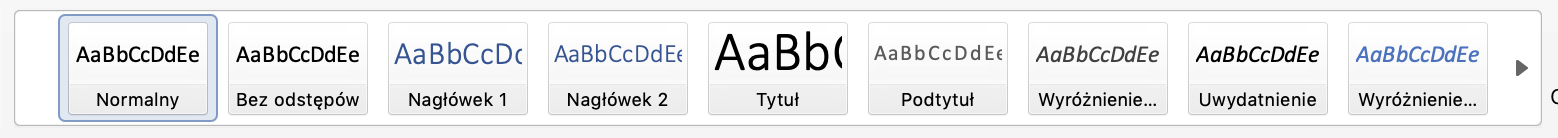
\includegraphics[width=\textwidth]{style}
        \caption{Pasek stylów w MS Word}
    \end{figure}
\end{center}


\subsection{Hierarchia treści, czyli tworzenie konspektu}
Widok konspektu jest rozwiązaniem oferowanym jedynie przez graficzne edytory tekstu takie jak MS Word. Oferuje on nam możliwość szybkiego i łatwego zmieniania kolejności rozdziałów i podrozdziałów w naszym tekscie. Również pozwala on na \emph{zagnieżdżanie} rozdziałów w sobie - zmienianie rozdziałów w podrozdziały. 

Dobrze wykonany konspekt nadaje dokumentom strukturę i sprawia, że dokument jest czytelniejszy. Zmiany w konspekcie powodują rownież zmiany w formatowaniu spowodowane przez wybrany styl.

\begin{center}
  \begin{figure}[h]
      \centering
      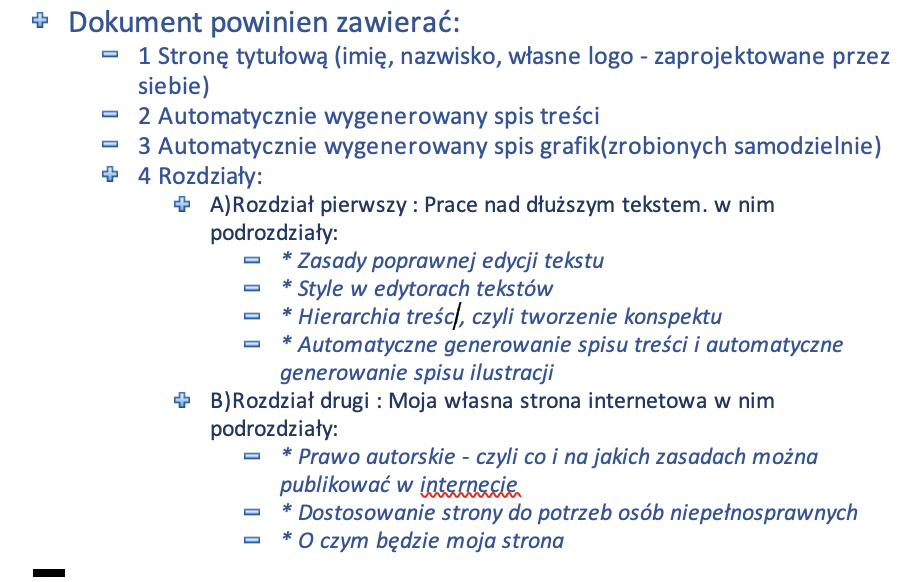
\includegraphics[scale=0.7]{konspekt}
      \caption{Poprawnie wykonany konspekt}
  \end{figure}
\end{center}

\begin{center}
  \begin{figure}[h]
      \centering
      
\includegraphics[scale=0.3]{efekt}
      \caption{Przykładowy efekt}
  \end{figure}
\end{center}

\newpage

\subsection{Automatyczne generowanie spisu treści i automatyczne generowanie spisu ilustracji}
Automatyczne generowanie spisu treści i spisu ilustracji w \LaTeX { }jest bardzo łatwe. Wystarczy napisać komendę \textbf{\textbackslash{tableofcontents}} w miejscu, w ktorym chcemy go wstawić. Analogicznie powstaje spis grafik - za pomocą komendy \textbf{\textbackslash{listoffigures}}
 \\

\section{Moja własna strona internetowa}
W tym rozdziale opowiem o mojej stronie internetowej, którą zamierzam opublikować pod \href{https://aszokalski.w.staszic.waw.pl}{tym adresem}. 
\subsection{Prawo autorskie - czyli co i na jakich zasadach można publikować w internecie}
Prawa autorskie służą do ochrony dzieł przed ich niesprawiedliwym udostępnianiem. Nie można w internecie opublikować kupionej książki ani za darmo, ani opdłatnie (mimo to ludzie to robią). Chyba, że autor na to wyraźnie zezwala. 

Autor ma prawo zezwolić na różne sposoby używania/rozprzestrzeniania jego dzieła oraz może na inne się nie zgodzić. Każde dzieło automatycznie podjęte jest pełną ochroną praw autorskich. Znaczy to, że każde niesprawiedliwe użycie dzieła może być karane. Jeśli autor jednak chce zezwolić w pewnym stopniu na udostępnianie/używanie jego pracy, może objąć ją odpowiednią uniwersalną licencją.

Te same zasady obejmują nie tylko książki, ale również: filmy, zdjęcia, teksty. Programy za to rządzą się trochę bardziej skomplikowanymi zasadami i zazwyczaj mają one wyraźne licencje.

\newpage

\subsection{Dostosowanie strony do potrzeb osób niepełnosprawnych}
Strony internetowe muszą być dostosowane do potrzeb osób niepełnosprawnych. Osoba niewidoma na przykład chciałaby usłyszeć je zawartość w formie audio. Seria wytycznych \textbf{Web Content Accessibility Guidelines} (WCAG) dokładnie opisuje jak dostoswoać stronę pod potrzeby osób niepełnosprawnych. Oto pewne konwencje, które warto zastosować:
\begin{itemize}
  \item{\textbf{Korzystanie z alt-tagów} - program czytający tekst przeczyta tekst opisujący obrazek }
  \item{\textbf{Transkrybowanie filmów} - z tego samego powodu }
  \item{\textbf{Mądre stosowanie kolorów} - najlepiej pozostać przy czarnym tekscie na białym tle, aby daltoniści nie mieli problemu z odczytaniem treści}
  \item{\textbf{Wyraźnie zaznaczaj linki i przyciski} - aby osoby słabo widzące mogły łatwo je namierzyć. Warto to robić nawet ze względu na osoby zdrowe}
  \item{\textbf{Dostosuj stronę pod nawigację z klawiatury} - bo nie każdy może korzystać z myszki}
\end{itemize}

\subsection{O czym będzie moja strona?}
Moja strona internetowa będzie moją internetową wizytówką. Planuję z niej zrobić czytelne i przejrzyste źródło informacji na temat moich działalności i projektów. Chciałbym też, żeby była wygodnym źródłem moich informaci kontaktowych.

\begin{thebibliography}{1}

  \bibitem{notes} Cognity \href{https://www.cognity.pl/15-zasad-poprawnego-formatowania-tekstu-wnbspms-word,blog,105.html}{\em 15 zasad poprawnego formatowania tekstu w MS Word}.

  \bibitem{notes} Denis Peszka \href{https://smartbees.pl/blog/dostosowanie-strony-www-dla-niepelnosprawnych-6-przydatnych-porad}{\em Dostosowanie www dla niepelnosprawnych}.
  
  \end{thebibliography}

\end{document}